%%%%%%%%%%%%%%%%%%%%%%%%%%%%%%%%%%%%%%%%
%% MCM/ICM LaTeX Template %%
%% 2024 MCM/ICM           %%
%%%%%%%%%%%%%%%%%%%%%%%%%%%%%%%%%%%%%%%%
\documentclass[12pt]{article}
\usepackage{geometry}
\geometry{left=1in,right=0.75in,top=1in,bottom=1in}

%%%%%%%%%%%%%%%%%%%%%%%%%%%%%%%%%%%%%%%%
% Replace ABCDEF in the next line with your chosen problem
% and replace 1111111 with your Team Control Number
\newcommand{\Problem}{A}
\newcommand{\Team}{2403424}
%%%%%%%%%%%%%%%%%%%%%%%%%%%%%%%%%%%%%%%%

\usepackage{newtxtext}
\usepackage{amsmath,amssymb,amsthm}
\usepackage{newtxmath} % must come after amsXXX
\usepackage[format=hang]{caption} % add support for caption*
\usepackage{cite}
\usepackage{graphicx}
\usepackage{xcolor}
\usepackage{fancyhdr}
\usepackage{listings}
\usepackage{xeCJK}



\definecolor{codegreen}{rgb}{0,0.6,0}
\definecolor{codegray}{rgb}{0.5,0.5,0.5}
\definecolor{codepurple}{rgb}{0.58,0,0.82}
\definecolor{backcolour}{rgb}{0.95,0.95,0.92}

\lstdefinestyle{mystyle}{
    backgroundcolor=\color{backcolour},   
    commentstyle=\color{codegreen},
    keywordstyle=\color{magenta},
    numberstyle=\tiny\color{codegray},
    stringstyle=\color{codepurple},
    basicstyle=\ttfamily\footnotesize,
    breakatwhitespace=false,         
    breaklines=true,                 
    captionpos=b,                    
    keepspaces=true,                 
    numbers=left,                    
    numbersep=5pt,                  
    showspaces=false,                
    showstringspaces=false,
    showtabs=false,                  
    tabsize=2
}

\lstset{style=mystyle}

\lhead{Team \Team}
\rhead{}
\cfoot{}

\newtheorem{theorem}{Theorem}
\newtheorem{corollary}[theorem]{Corollary}
\newtheorem{lemma}[theorem]{Lemma}
\newtheorem{definition}{Definition}
%%%%%%%%%%%%%%%%%%%%%%%%%%%%%%%%
\begin{document}
\graphicspath{{.}}  % Place your graphic files in the same directory as your main document
\DeclareGraphicsExtensions{.pdf, .jpg, .tif, .png}
\thispagestyle{empty}
\vspace*{-16ex}
\centerline{\begin{tabular}{*3{c}}
		\parbox[t]{0.3\linewidth}{\begin{center}\textbf{Problem Chosen}\\ \Large \textcolor{red}{\Problem}\end{center}}
		 & \parbox[t]{0.3\linewidth}{\begin{center}\textbf{2024\\ MCM/ICM\\ Summary Sheet}\end{center}}
		 & \parbox[t]{0.3\linewidth}{\begin{center}\textbf{Team Control Number}\\ \Large \textcolor{red}{\Team}\end{center}} \\
		\hline
	\end{tabular}}
%%%%%%%%%%% Begin Summary %%%%%%%%%%%
% Enter your summary here replacing the (red) text
% Replace the text from here ...
\begin{center}
	\textbf{\Huge Lamprey: A New Model for the Spread of an Invasive Species}
	\begin{figure}[h]
		\centering
		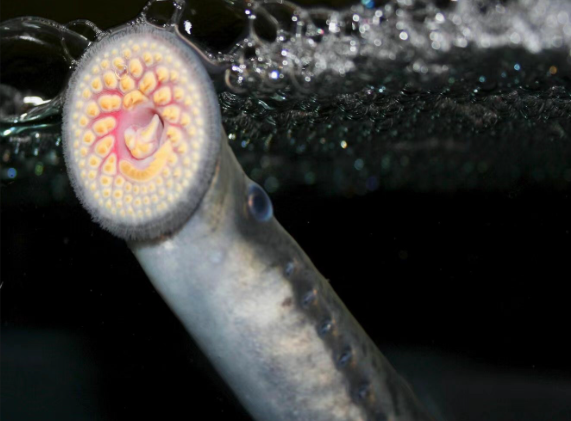
\includegraphics[width=0.7\textwidth]{LampreyFigure.png}
		\caption{Lamprey by Great Lakes Science Center\cite{sea-lamprey-2}.}
	\end{figure}
	% real summary beginning
\end{center}
\quad As a powerful invasive species in the Great Lakes from the 1940s, lamprey populations are 
closely linked to the entire Great Lakes ecosystem. The female propotion of lampreys is positively 
correlated with the growth rate in their larval stages, and the growth rate of these larvae is affected 
by the amount of available food resources. The purpose of this study was to establish an analytical model 
to simulate the reproductive activities of lampreys under the influence of sex ratio changes and to 
evaluate the impact of sex ratio change mechanisms on lamprey offspring. We also build models of 
interactions between lampreys and other species to analyze the relationship between lamprey population 
development and ecosystems. \\
\quad In the study, we used a total of three models; \\
\textbf{Model 1}: Lotka-Volterra model that introduced gender change factors;\\
\textbf{Model 2}: Lamprey's body shape-first mate selection strategy and reproduction model;\\
\textbf{Model 3}: Based on the multi-species Lotka-Volterra model Matrix iteration model. \\
\quad We hope this study will help optimize the control of lampreys in the Great Lakes, and provide assistance in studying the reproductive activities of lamprey populations.
% to here
%%%%%%%%%%% End Summary %%%%%%%%%%%
\newpage
\tableofcontents
\newpage
%%%%%%%%%%%%%%%%%%%%%%%%%%%%%%
\clearpage
\pagestyle{fancy}
% Uncomment the next line to generate a Table of Contents
%\tableofcontents 
\newpage
\setcounter{page}{1}
\rhead{Page \thepage\ }
%%%%%%%%%%%%%%%%%%%%%%%%%%%%%%


%%%%%%%%%%%%%%%%%%%%%%%%%%%%%%
\section{Introduction}
\subsection{Problem Background}
\quad Sea lampreys in the Great Lakes basin exhibit sex ratio variation that adapts to environmental conditions.
The Great Lakes ecosystem has seen fluctuations in lamprey populations, with the sex ratio influenced by
the growth rates in their larval stages, which are contingent upon food availability. In environments with
limited food, a slower growth rate skews the population toward a higher male ratio up to 78\%. Conversely,
with better food availability, the male percentage decreases to approximately 56\%. The sex ratio adaptation
in sea lampreys affects prey species, lamprey populations, and competition dynamics between lamprey and other
species within the Great Lakes. The ability to adjust sex ratios allows lampreys to potentially stabilize
their population in varying conditions, influencing the broader ecosystem balance.
\section{Approach to Problem Solving}
\quad The purpose of our research on the lamprey involves studying the effects of altered sex ratios on the ecosystem,
evaluating the consequences for lamprey populations, and understanding the broader implications for ecosystem
stability. We aim to determine how these changes might benefit or harm other species, including parasites.
\\
Utilizing population structure data of lampreys, trout, and salmon from the Great Lakes, we have revised the
Lotka-Volterra competition model by incorporating a sex ratio factor. We employed the Monte Carlo method to
examine two alternative mating strategies beyond traditional monogamy, exploring how sex ratio skews—though
seemingly detrimental to population size—persist through genetic and evolutionary mechanisms. Our analysis
confirmed a link between sex ratio shifts and increases in individual size and survival capabilities.
\\
We developed a Great Lakes resource transfer model using matrix iteration and applied the predation aspect
of the Lotka-Volterra model to simulate and measure ecosystem stability, utilizing system time-domain
indicators to evaluate stability levels. This analysis was further enhanced by incorporating genetic
perspectives and species richness.
\\
Incorporating the multi-species form of the Lotka-Volterra equation and a resource transfer matrix, we
described the direct and indirect interactions within the entire food chain. We elucidated the role of
lampreys as a keystone component of the ecosystem, functioning as parasite carriers, nest builders,
and parasites themselves, and demonstrated how the unique reproductive trait of sex ratio alteration
impacts other ecosystem components.
\section{General Assumptions and Model Overview}
To simplify the problem, we make the following basic assumptions.
\subsection*{Model Preparation}
\subsubsection*{Notation}
\subsubsection*{Data}
Redd superimposition mediates the accuracy, precision, and significance of redd counts for cutthroat trout\\
Relation of Sea Lamprey Size and Sex Ratio to Salmonid Availability in Three Great Lakes \\
SEA LAMPREY CONTROL IN THE GREAT LAKES 2020 \\
Relation of Sea Lamprey Size and Sex Ratio to Salmonid Availability in Three Great Lakes \\
Quantifying Great Lakes sea lamprey populations using an index of adults\\
A review of sea lamprey dispersal and population structure in the Great Lakes and the implications for control \\
\subsubsection*{Data Cleaning}
\subsection{Q1}
\subsubsection{Reason for Choosing the Lotka-Volterra Model}
In the Great Lakes, sea lampreys exist in an advantageous habitat with virtually no natural predators. 
The ecological relationships primarily associated with sea lampreys are predation (parasitism) on other 
fish species and competition. We need to mathematically represent these two types of ecological 
relationships, with consideration for both time and resource availability dimensions in terms of 
population numbers. Hence, we introduce the Lotka-Volterra model.\\
The Lotka-Volterra model typically describes the interrelationships between two or more biological 
populations. In our application, we represent all species competing with the sea lamprey as a single 
unit. This approach simplifies the model to a certain extent, though omitting some ecological 
relationships. Of course, our research aims for the model to be applicable to a larger ecosystem, 
including the multiple species found in the Great Lakes, making such simplifications reasonable. 
\subsubsection{Introducing a Sex Ratio Change Factor}
In both the Competitive Lotka-Volterra Model and the Lotka-Volterra Predator-Prey Model, changes 
in population numbers are related to the populations of both partie, numerically equal to the 
quantity of the two population numbers multiplied by some coefficient. However, in traditional 
Lotka-Volterra models, the birth rate of a species is set as a constant. For lampreys, when the 
proportion of females is affected by a reduction in food during the juvenile stage, deviating 
from a 0.5 ratio, the birth rate will decrease. Then setting the birth rate as a constant will 
be unreasonable. To correct this deviation, we have modified the coefficients of the model and 
introduced a sex ratio factor to depict the decline in birth rate.  
\begin{figure}[h]
	\large
	\centering
	$\frac{dx}{dt}=\alpha x - \beta xy$ \\
	$\frac{dy}{dt}=\delta xy - \gamma y$
	\caption*{Lotka-Volterra predator-prey model}
\end{figure}

\begin{figure}[h]
	\large
	\centering
	$\frac{dx_1}{dt}=r_1x_1(1-(\frac{x_1+\alpha_{12}x_2}{K_1}))$ \\
	$\frac{dx_2}{dt}=r_2x_2(1-(\frac{x_2+\alpha_{21}x_1}{K_2}))$
	\caption*{Competitive Lotka-Volterra model}
\end{figure}
In both models, we introduced the term $\frac{dR_f}{dt}$, which describes the impact on the birth 
rate as the female ratio declines. When the proportion of females continues to decrease, the 
birth rate should also decrease accordingly. Considering that the birth rate and sex ratio are 
two completely different types of data, we have also applied a certain coefficient to this factor 
in order to match it with real-world data, thereby providing a more accurate description of the 
actual situation. 
\subsection*{Description of Available Food Quantity}
In the Competitive Lotka-Volterra Model, the quantity of available food is not directly reflected 
in the equations. However, the amount of food is positively correlated with the carrying 
capacity $K$, so in our formulation, we have modified the constant $K$ to be a variable that 
diminishes over time with small random changes.  
\subsubsection{Analysis and Conclusion}
\begin{figure}[h]
	\centering
	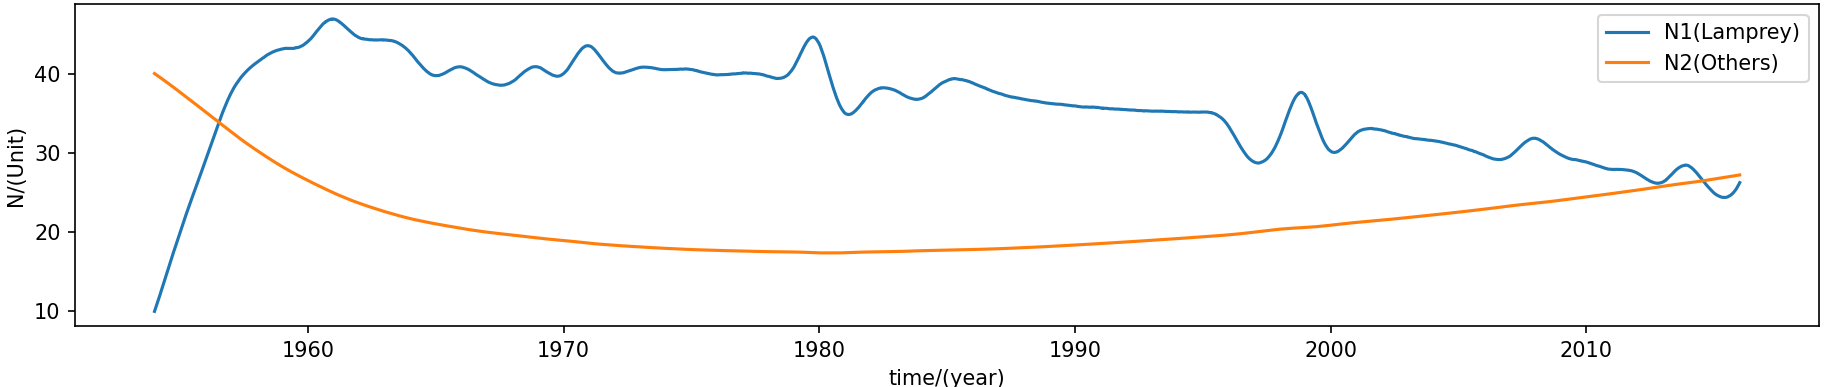
\includegraphics[width=0.9\textwidth]{Q1_LVComp.png}
	\caption{The relationship between the proportion}
\end{figure}
\begin{figure}[h]
	\centering
	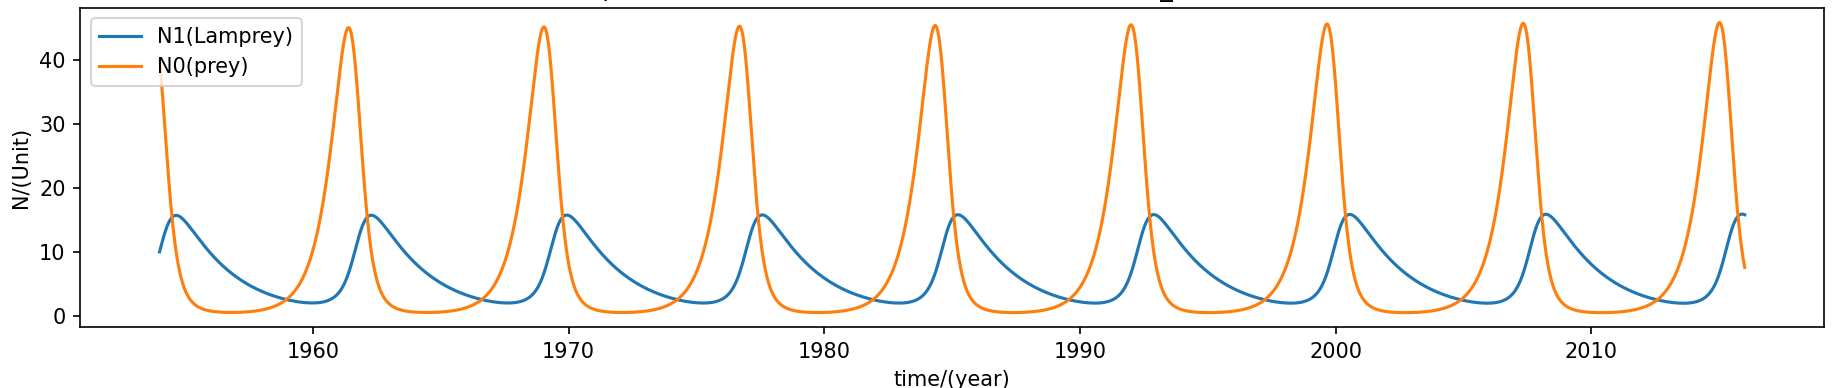
\includegraphics[width=0.9\textwidth]{Q1_LVPP.png}
	\caption{The relationship between the proportion}
\end{figure}
In our research, we used trout and salmon as examples of species [ 公式 N2 ] $N_2$in the predation 
formula, as these species have a significant presence in the diet of sea lampreys in the Great Lakes. 
In the competition formula, we did not design specific examples, but rather treated the species 
competing with the lamprey as a generalized whole. \\
In the figures, it can be observed that in the competitive model, the initially disadvantaged 
lamprey managed to surpass the numbers of its competitors by reducing its offspring generation 
in the first few generations and thereby relieving survival pressure for the future. From the 
perspective of the macro ecosystem, the sea lamprey, as an invasive species, has somewhat 
enhanced its adaptability to the environment through the ability to alter its sex ratio, 
which facilitates environmental adaptation and dominance in the food chain, thereby invading 
new areas and expanding the influence of the sea lamprey. \\
Additionally, as will be described in later sections of the article, the sea lamprey's survival 
ability and body size increase as the birth rate decreases, leading to a greater suppressive 
effect on other species and a stronger influence on its prey. Consequently, this exerts more 
significant pressure on other species. From the perspective of ecological niches, a certain 
level of harsh environment is actually beneficial for the sea lamprey population. The prosperity 
of the sea lamprey population creates a crowding-out effect on its competitors. 
Although no species have been found to rapidly decline in numbers due to the sea 
lamprey based on actual statistical data, the growth in the sea lamprey population has undoubtedly 
impacted the Great Lakes ecosystem. \\
As an invasive species, the gender transition mechanism of the lamprey has enabled the population 
to access more abundant resources and a broader ecological niche, significantly impacting the 
original food chains of the Great Lakes. This includes the suppression of predatory fish and 
parasites and a decrease in the number of large fish hosts, which struggle to reach full 
development under the lamprey problem. Such phenomena could potentially lead to reduced 
biodiversity and damage the original ecological balance of the ecosystem. However, considering 
the near-stable performance of the Great Lakes ecosystem from the 1940s to the present, it is 
possible that the presence of the lamprey has also established a new ecological equilibrium. 
\subsection{Q2}
In this problem, we focus on the mate selection of lampreys, and we will explain that the mate 
selection strategy will have an important impact on the offspring individuals in the 
population in the context of changing sex ratio.
\subsubsection{Reasons for using Monte Carlo Method}
Monte Carlo method allows us to assume some individuals and directly simulate the mating between 
these individuals, and then simulate the distribution of some of their characteristics. 
Monte Carlo method is very intuitive, and often matches well with the statistics of small 
range of marking method, because the Monte Carlo process is close to the real reproductive process. 
\subsubsection{Two Different Mating Strategies}
Consider two different strategies to expand the traditional monogamous mating. Note that the 
male lamprey has a limited number of reproductive times, and the female lamprey mostly has 
only one child, which means a female often sham mates with some males, and chooses another 
one as the final father. Our code sets the number of reproductive times of the male lamprey 
as up to five times, with different success rates for different reproductive times; the female 
lamprey steadily has one child. In the two simulated mating strategies, the first strategy is 
the "smart female" mating strategy: under this strategy, the female lamprey will only choose 
the mating partner with the largest size. The second strategy is the "probabilistic female" 
mating strategy, in which the female lamprey will accept the mating offer with a corresponding 
probability according to the size of the male lamprey. If the male body size is less than 
half of the female body size, it is rejected directly; if the male body size is between half 
of the female body size and the female body size, a probability based on the size difference 
is accepted; if the male body size is greater than the female body size, the probability of acceptance is higher. 
\subsubsection{Two different forms of generation}
The modeling considers two forms of generation and two mating strategies.The first form of 
generation is simple, and the size of the offspring is the average of the maternal size 
plus a random amount.Because the growth process is very complex, the average method will 
be most realistic.The second form of generation considers the genotype (in the case of 
dominant genes, and the same for recessive genes).This can focus on the selection effect 
of mating strategies on a specific gene. \\
In either case, the probability of a larger mother producing larger offspring is higher 
than that of a smaller mother. 
\subsubsection{Female lamprey mating}
It can be found that in most lamprey populations, female lampreys are less than male lampreys, 
and females have the opportunity to select males in terms of body size and pheromone. In the 
case of more imbalanced sex ratio, female selection will be more strict, and the larger 
size of the male will have the priority of mating, and the size of the offspring will 
also increase with each generation. \\
In the model, with the change of the larval growth resources, the female proportion will 
further decrease, and the stronger the selection of the male will be: the smaller proportion 
of the larger size of the male will have the opportunity to reproduce the offspring, and the 
size of the offspring will also increase. 
\subsubsection{Impact on the lamprey population }
Advantages: 1. According to the model, we can find that the lamprey's ability to change 
the sex ratio can make the population of the offspring have a larger size. And according 
to the study [ link, superscript form ], a larger size is conducive to the migration and 
spawn. 2. The energy consumed by the male to mature and produce sperm is less than that of 
the female to mature and produce eggs, and the lamprey population with a higher proportion of 
males can more easily adapt to the environment of scarcity.\\
Disadvantages: If the second generation is produced, it is clear that the S gene frequency 
of the offspring will exceed the s gene frequency, and the s gene frequency may become 
very small after many generations. This shows that the gene diversity of the lamprey 
is reduced, which is not conducive to the population to cope with the mutated environment. 
\subsection{Q3}
\subsubsection{Reasons for choosing resource transfer matrix}
In Lotka-Votterra model, if multiple species are considered, the interactions between species 
will form an influence matrix. If we are not limited to predation relationships, but put all 
kinds of resource transfer in a matrix, we will get a resource transfer matrix. This matrix 
describes how species obtain resources such as food or reusable nests from other species.\\
The resource transfer matrix can describe the direct or indirect influences between various 
components of the whole ecosystem, give the ecological niche of lamprey in the ecosystem, 
and clearly reflect the material transfer and energy flow between organisms. 
\subsubsection{Model interpretation}
\begin{figure}[h]
	\centering
	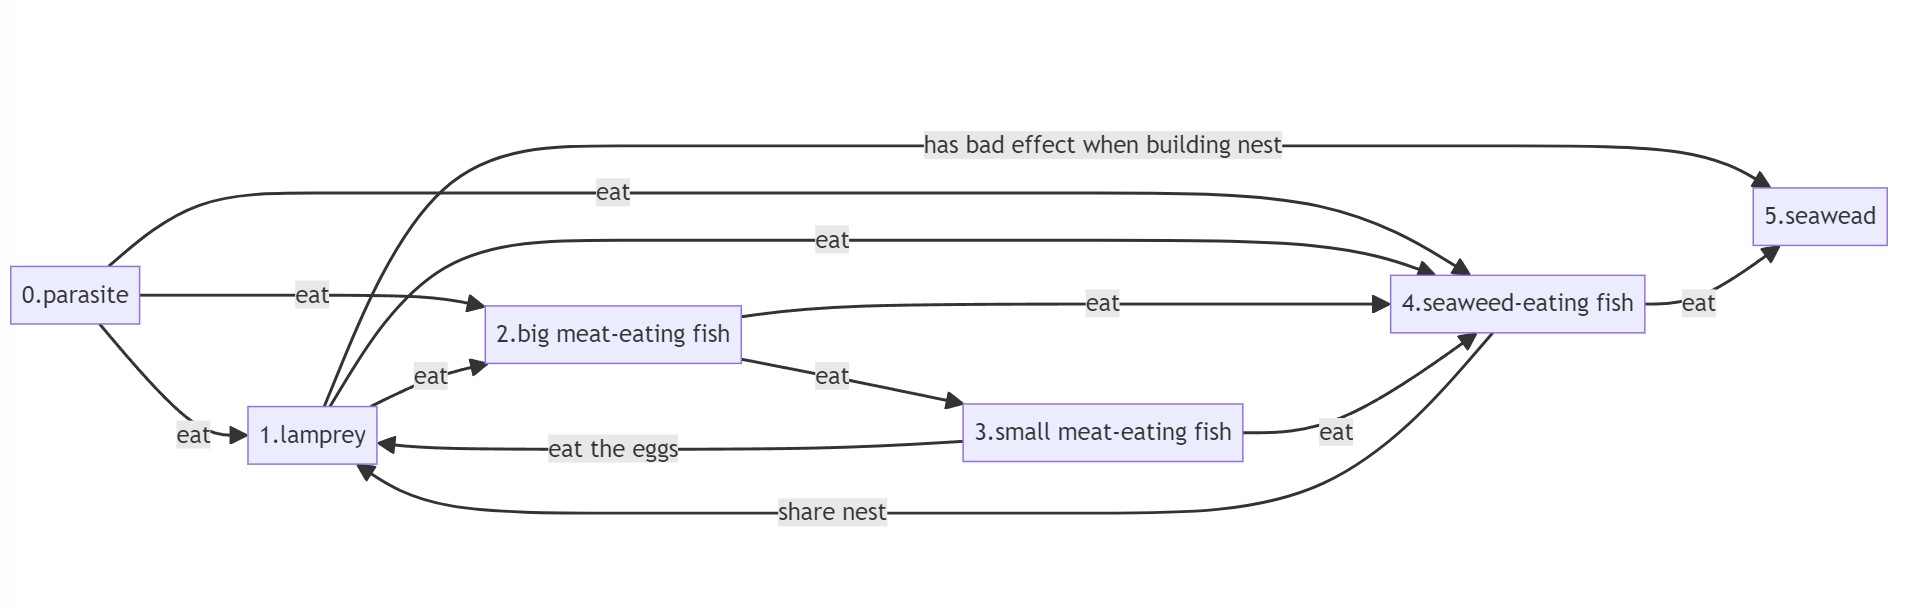
\includegraphics[width=0.9\textwidth]{Q4_EnvStructure.png}
	\caption{Resource transfer diagram}
\end{figure}
\begin{figure}[h]
	\centering
	$\begin{pmatrix}
			A_{11} & A_{12} & A_{13} & A_{14} & A_{15} & A_{16} \\
			A_{21} & A_{22} & A_{23} & A_{24} & A_{25} & A_{26} \\
			A_{31} & A_{32} & A_{33} & A_{34} & A_{35} & A_{36} \\
			A_{41} & A_{42} & A_{43} & A_{44} & A_{45} & A_{46} \\
			A_{51} & A_{52} & A_{53} & A_{54} & A_{55} & A_{56} \\
			A_{61} & A_{62} & A_{63} & A_{64} & A_{65} & A_{66}
		\end{pmatrix}$
	\caption*{Example of a resource transfer matrix}
\end{figure}
If an connection is drawn in the diagram, like the connection between (3.small carnivarous 
fish) and (1.lamprey), we put a positive coefficient in the matrix, for $A_{31} = 0.1$. 
We build the matrix all by the diagram in this way. \\
We can see that, in the resource transfer diagram, most relationships are based on predation. 
These relationships do not have a direct connection to lamprey's ability to change sex, but 
they are essential within the ecosystem.\\
Other factors are related to lamprey's sex change and reproduction. For instance, some parasites, 
in addition to inhabiting lampreys, may also use lampreys as carriers. Carrier activities are 
often associated with the lamprey's migratory behavior and the release of traceable pheromones 
during their mating activities. Parasites can locate lampreys based on these pheromones and 
can attach themselves to migrating lampreys to travel long distances. Another example is that 
some small animals may use the nests of lampreys, which is closely related to the sex ratio of 
lampreys, as nest-building activities are initiated by males, and the proportion of males will 
affect the number of nests available. 
\subsubsection{Analysis of Results}
It can be observed intuitively that there are periodic fluctuations in the population numbers in 
both graphs. However, when the interaction coefficient between lampreys and other species is 
reduced, the entire system becomes more unstable, and the amplitude of fluctuations increases 
with the simulation time. This suggests that the existence of the sex-changing mechanism in 
lampreys can generate more resources for other organisms to utilize, thereby enhancing the 
stability of the ecosystem.\\
When considering the actual situation, we find that males bear the burden of nest building, and 
these nests can be utilized by other organisms. Additionally, according to the conclusion 
from Q2, changes in the sex ratio are advantageous for producing individuals with stronger 
migratory capabilities and more pheromones. This can attract and carry more parasites, from 
which the parasites will benefit.
\subsubsection{Impact on Ecosystem Stability}
\begin{figure}[h]
	\centering
	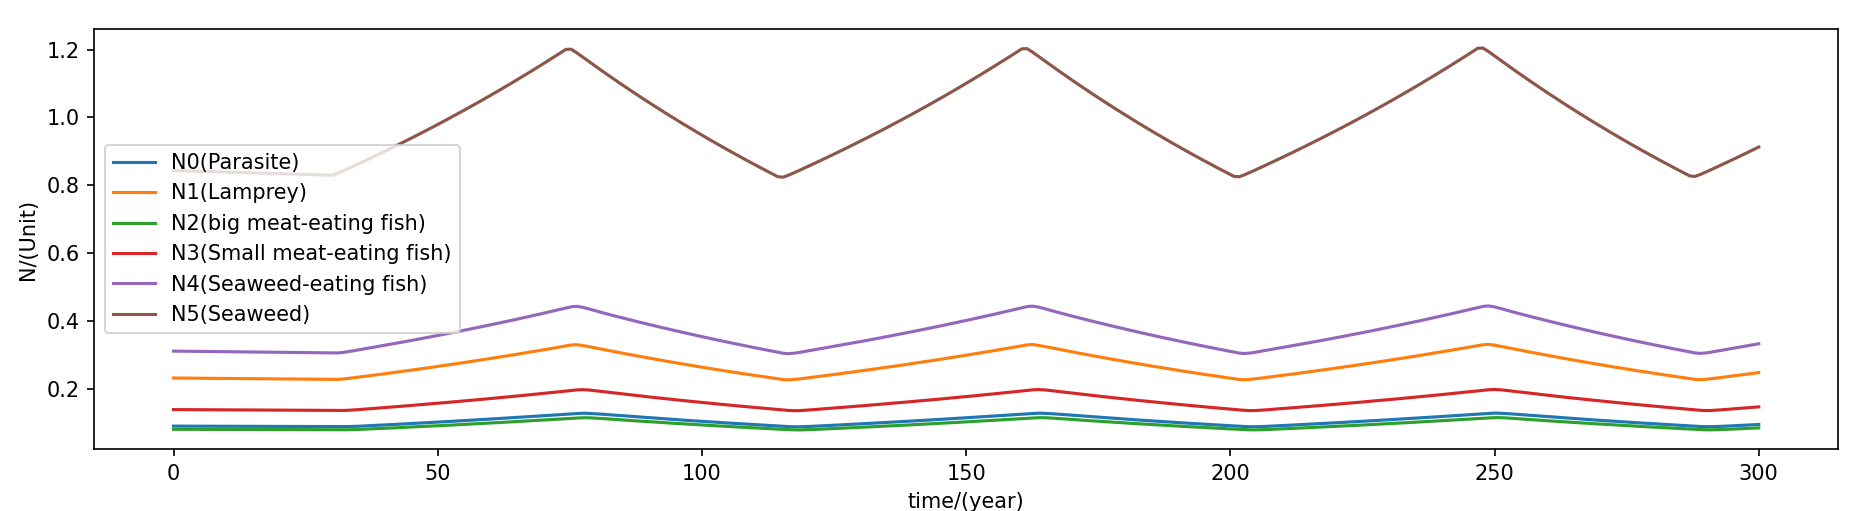
\includegraphics[width=0.9\textwidth]{Q3_divergent.png}
	\caption{divergent model}
\end{figure}
\begin{figure}[h]
	\centering
	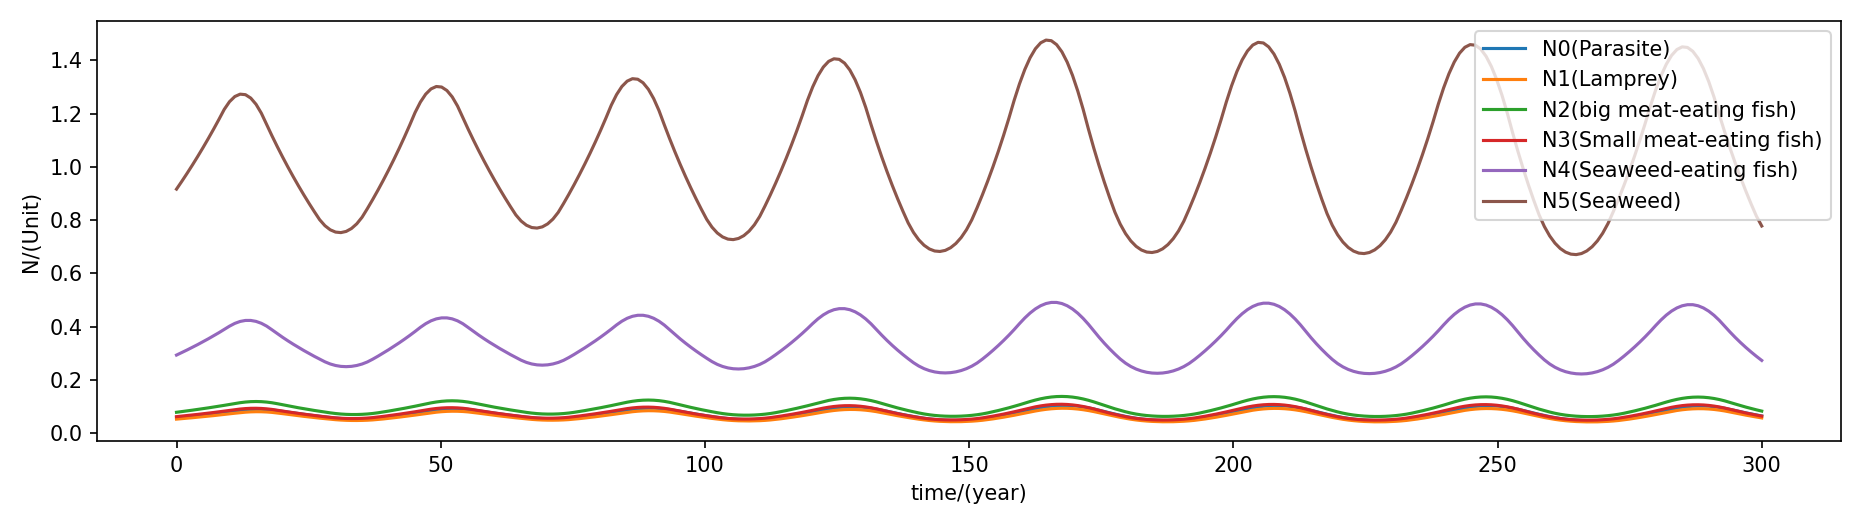
\includegraphics[width=0.9\textwidth]{Q3_nondivergence.png}
	\caption{nondivergent model}
\end{figure}
Advantages: Firstly, after the sea lamprey is introduced into an ecosystem, its gene pool becomes 
a part of the ecosystem's gene pool, enriching the genetic diversity to a certain extent. 
Secondly, after the sea lamprey invades the ecosystem for a while, the ecosystem will reach 
a new steady state. The sex-changing ability of the sea lamprey enables its population to 
be relatively well-preserved under various conditions. Thirdly, the sea lamprey population 
has a higher proportion of males after sex change, which requires fewer resources, and 
outputs more available resources to other organisms, which is beneficial for the ecosystem stability.\\
Disadvantages: Firstly, the sex-changing ability of the sea lamprey allows it to invade ecosystems 
more quickly and occupy important ecological niches. This will inevitably lead to a sharp decline 
in the numbers of some local species due to predation or competition, threatening them with 
extinction or even leading to their demise, which undoubtedly disrupts species diversity. 
Secondly, when sea lampreys change their sex ratio, reducing mating and offspring production, 
their genetic diversity is reduced, and the genetic reservoir of the ecosystem will also shrink. 
This is detrimental to ecosystem stability. 
\subsection{Q4}
\subsubsection{Model Selection}
In this module, we continue to use the resource transfer matrix model. When constructing the model 
in Q3, we added a specific element for parasites, allowing us to observe the amplitude and frequency 
of the cyclical changes in parasite population numbers. 
\subsubsection{Analysis of Results}
Due to the mechanism of sex change in lampreys, males will have much more males than females in 
situations of lack of resources, thus leading to very fierce competition. Males release pheromones 
to attract females to sexual intercourse, and pheromones can act as a stimulus for some parasites 
to locate lampreys, providing them with more hosts.\\
In addition, we also revealed in Q2 that the change in sex ratio is conducive to the production 
of more migratory offspring, which is conducive to the carriage of parasites.The survival of 
parasites is closely related to the sex ratio of octopods. 
\section{Further Research}
1.The genes that control body size are likely to be multiple alleles rather than a single one.
Therefore, our genetic model requires more data and more refined simulation.
\section{Conclusion}
\newpage
%Appendices 
\newpage
\listoffigures
\listoftables
\bibliography{library,images}
\bibliographystyle{plain}
\newpage
\section*{Appendices}
\subsection*{Program for Q1}
\lstinputlisting[language=Python]{../Src/Q1.py}
\lstinputlisting[language=Python]{../Src/Q1_2.py}
\subsection*{Program for Q2}
\lstinputlisting[language=Python]{../Src/Q2_1.py}
\lstinputlisting[language=Python]{../Src/Q2_2.py}
\lstinputlisting[language=Python]{../Src/Q2_3.py}
\subsection*{Program for Q3, Q4}
\lstinputlisting[language=Python]{../Src/Q3-Q4.py}
%%%%%%%%%%%%%%%%%%%%%%%%%%%%%%
\end{document}
